\documentclass{article}
\usepackage{tikz}
\usepackage[english]{babel}
\usepackage{graphicx}
\usepackage{float}
\usetikzlibrary{positioning,arrows}
\usepackage{pgfplots}
\usepackage{amsmath}
\usepackage{amsfonts}
\pgfplotsset{compat=1.12}
\usepackage[utf8]{inputenc}

\usepackage[numbers]{natbib}
\usepackage{enumerate}
\usepackage[margin=1.0in]{geometry}

\usepackage{natbib}

\title{Report}
\author{vamshi kammadanam}
\date{July 2015}




\begin{document}

\maketitle

\section{Physical Layer}
The idea is to implement cryptographic scheme at physical layer. However, due to limited resources available the cryptographic primitive should be modified/changed to suit the need without compromising security. The implementation requires understanding the standard physical layer and the resources available. In this respect, we need to input about the standard physical layer and the resources available.

\section{Results from Simulation}
Analysis for BEC, BSC and AWGN channel. Will be adding more results in the case of AWGN channel. The red color indicates the results from \cite{arikan2008performance}. Blue color are the simulation results.

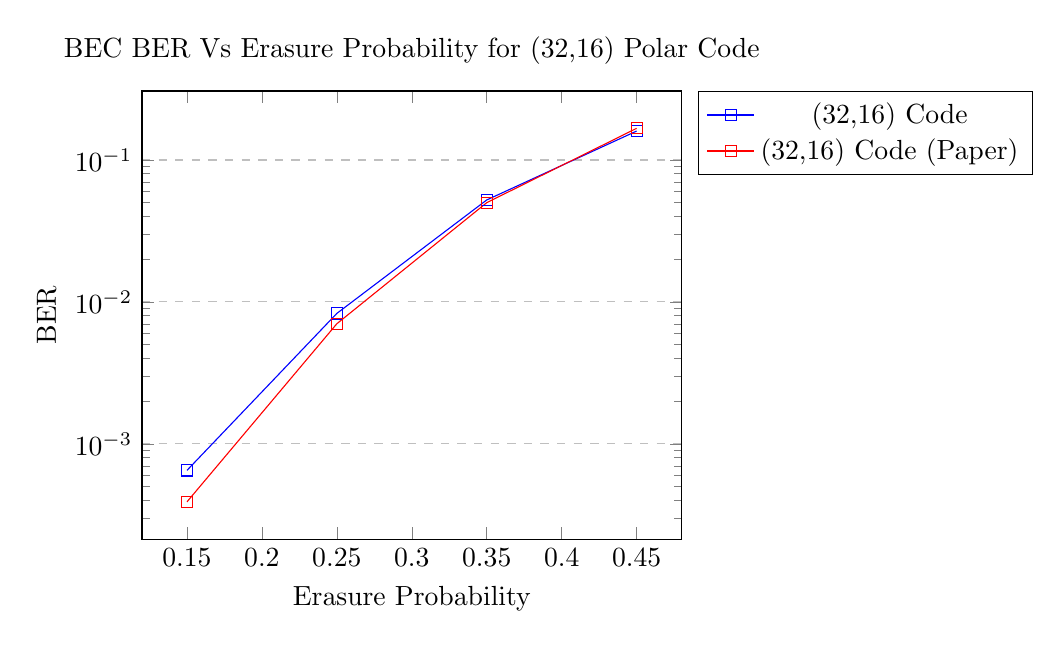
\begin{tikzpicture}
\begin{semilogyaxis}[
    title={BEC BER Vs Erasure Probability for (32,16) Polar Code},
    xlabel={Erasure Probability},
    ylabel={BER},
    % xmin=0, xmax=0.5,
    % ymin=0, ymax=0.2000,
    % xtick={0.05,0.15,0.25,0.35,0.45},
    % ytick={0.0000,0.0010,0.0083,0.0528,0.1600},
    legend pos=outer north east,
    ymajorgrids=true,
    grid style=dashed,
]
 
\addplot[
    color=blue,
    mark=square,
    ]
    coordinates {
    (0.05,0.0000)(0.15,0.00065)(0.25,0.0083)(0.35,0.0523)(0.45,0.1600)
    };
    \addlegendentry{(32,16) Code}
    
\addplot[
    color=red,
    mark=square,
    ]
    coordinates {
    (0.05,0.0000)(0.15,0.00039)(0.25,0.00702)(0.35,0.05005)(0.45,0.16722)
    };
    \addlegendentry{(32,16) Code (Paper)}
 
\end{semilogyaxis}
\end{tikzpicture}

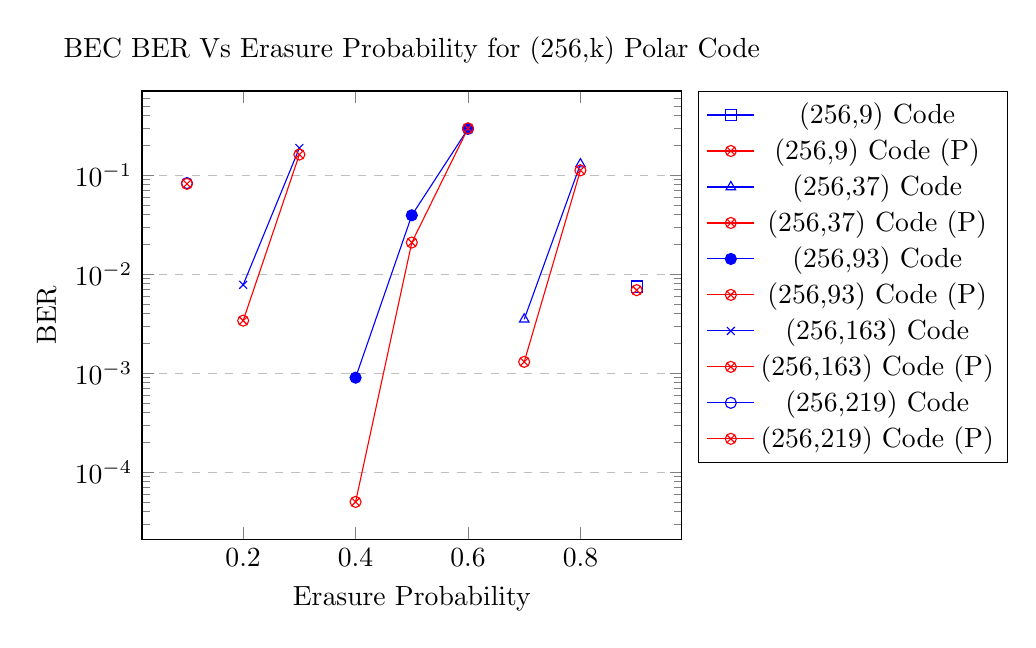
\begin{tikzpicture}
\begin{semilogyaxis}
[
    title={BEC BER Vs Erasure Probability for (256,k) Polar Code},
    xlabel={Erasure Probability},
    ylabel={BER},
    % xmin=0, xmax=1.0,
    % ymin=0, ymax=0.5000,
    % xtick={0.10,0.20,0.30,0.40,0.50,0.60,0.70,0.80,0.90,1.00},
    % ytick={0.00,0.050,0.100,0.150,0.250,0.300,0.350,0.400,0.450,0.500},
    legend pos=outer north east,
    ymajorgrids=true,
    grid style=dashed,
]
 
    \addplot[
    color=blue,
    mark=square,
    ]
    coordinates {
    (0.10,0.00)(0.20,0.00)(0.30,0.00)(0.40,0.00)(0.50,0.00)(0.60,0.00)(0.70,0.00)(0.80,0.00)(0.90,0.0075)
    };
    \addlegendentry{(256,9) Code}
    
    \addplot[
    color=red,
    mark=otimes,
    ]
    coordinates {
    (0.10,0.00)(0.20,0.00)(0.30,0.00)(0.40,0.00)(0.50,0.00)(0.60,0.00)(0.70,0.00)(0.80,0.00)(0.90,0.00689)
    };
    \addlegendentry{(256,9) Code (P)}
    

    \addplot[
    color=blue,
    mark=triangle,
    ]
    coordinates {
    (0.10,0.00)(0.20,0.00)(0.30,0.00)(0.40,0.00)(0.50,0.00)(0.60,0.00)(0.70,0.0035)(0.80, 0.1293)
    };
    \addlegendentry{(256,37) Code}
    
    \addplot[
    color=red,
    mark=otimes,
    ]
    coordinates {
    (0.10,0.00)(0.20,0.00)(0.30,0.00)(0.40,0.00)(0.50,0.00)(0.60,0.00)(0.70,0.00130)(0.80, 0.11181)
    };
    \addlegendentry{(256,37) Code (P)}
    
    \addplot[
    color=blue,
    mark=*,
    ]
    coordinates {
    (0.10,0.00)(0.20,0.00)(0.30,0.00)(0.40,0.0009)(0.50,  0.0393)(0.60,0.2934)
    };
    \addlegendentry{(256,93) Code}
    
    \addplot[
    color=red,
    mark=otimes,
    ]
    coordinates {
    (0.10,0.00)(0.20,0.00)(0.30,0.00)(0.40,0.00005)(0.50,  0.02087)(0.60,0.29740)
    };
    \addlegendentry{(256,93) Code (P)}
    
    \addplot[
    color=blue,
    mark=x,
    ]
    coordinates {
    (0.10,0.00)(0.20,0.0078)(0.30, 0.1879)
    };
    \addlegendentry{(256,163) Code}
    
    \addplot[
    color=red,
    mark=otimes,
    ]
    coordinates {
    (0.10,0.00)(0.20,0.00339)(0.30, 0.16155)
    };
    \addlegendentry{(256,163) Code (P)}
 
    \addplot[
    color=blue,
    mark=o,
    ]
    coordinates {
    (0.10,0.0832)
    };
    \addlegendentry{(256,219) Code}
    
    \addplot[
    color=red,
    mark=otimes,
    ]
    coordinates {
    (0.10,0.08167)
    };
    \addlegendentry{(256,219) Code (P)}
    
\end{semilogyaxis}
\end{tikzpicture}



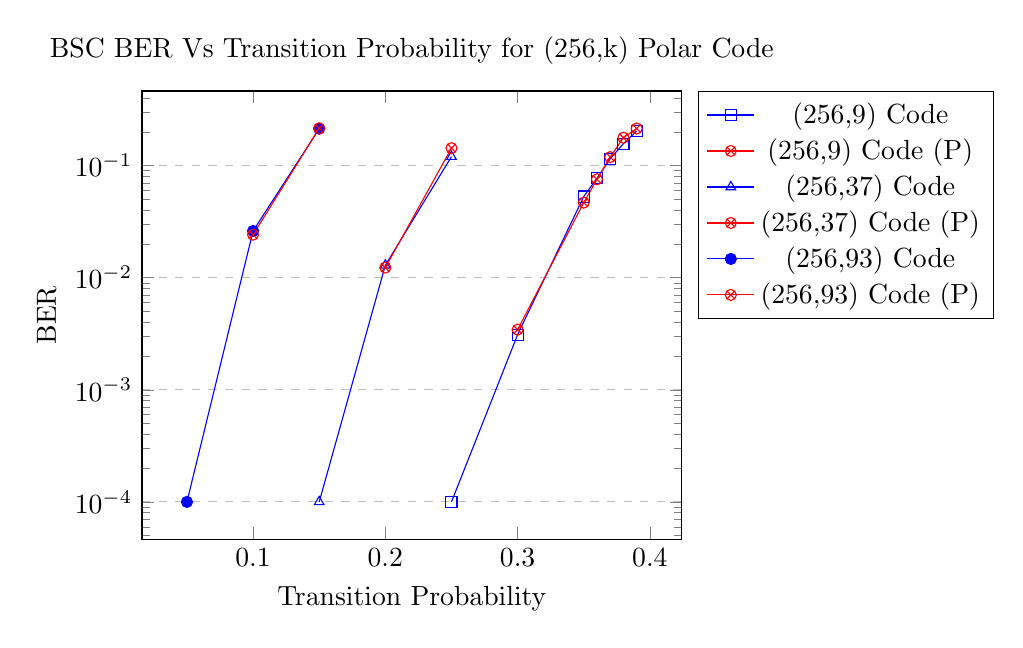
\begin{tikzpicture}
\begin{semilogyaxis}
[
    title={BSC BER Vs Transition Probability for (256,k) Polar Code},
    xlabel={Transition Probability},
    ylabel={BER},
    % xmin=0, xmax=1.0,
    % ymin=0, ymax=0.5000,
    % xtick={0.10,0.20,0.30,0.40,0.50,0.60,0.70,0.80,0.90,1.00},
    % ytick={0.00,0.050,0.100,0.150,0.250,0.300,0.350,0.400,0.450,0.500},
    legend pos=outer north east,
    ymajorgrids=true,
    grid style=dashed,
]
 
    \addplot[
    color=blue,
    mark=square,
    ]
    coordinates {
    (0.05,0.00)(0.10,0.00)(0.15,0.00)(0.20,0.00)(0.25,0.0001)(0.30,0.0031)(0.35,0.0529)(0.36,0.0771)(0.37,0.1146)(0.38,0.1568)(0.39,0.2029)
    };
    \addlegendentry{(256,9) Code}
    
    \addplot[
    color=red,
    mark=otimes,
    ]
    coordinates {
    (0.05,0.00)(0.10,0.00)(0.15,0.00)(0.20,0.00)(0.25,0.000)(0.30,0.00344)(0.35,0.04667)(0.36,0.07544)(0.37,0.11889)(0.38,0.17722)(0.39,0.21378)
    };
    \addlegendentry{(256,9) Code (P)}
    

    \addplot[
    color=blue,
    mark=triangle,
    ]
    coordinates {
    (0.05,0.00)(0.10,0.00)(0.15,0.0001)(0.20,  0.0129)(0.25,  0.1201)
    };
    \addlegendentry{(256,37) Code}
    
    \addplot[
    color=red,
    mark=otimes,
    ]
    coordinates {
    (0.05,0.00)(0.10,0.00)(0.15,0.000)(0.20,  0.01230)(0.25,  0.14297)
    };
    \addlegendentry{(256,37) Code (P)}
    
    \addplot[
    color=blue,
    mark=*,
    ]
    coordinates {
    (0.05,0.0001)(0.10,  0.0261)(0.15,  0.2131)
    };
    \addlegendentry{(256,93) Code}
    
    \addplot[
    color=red,
    mark=otimes,
    ]
    coordinates {
    (0.05,0.000)(0.10,  0.02418)(0.15,  0.21481)
    };
    \addlegendentry{(256,93) Code (P)}

\end{semilogyaxis}
\end{tikzpicture}

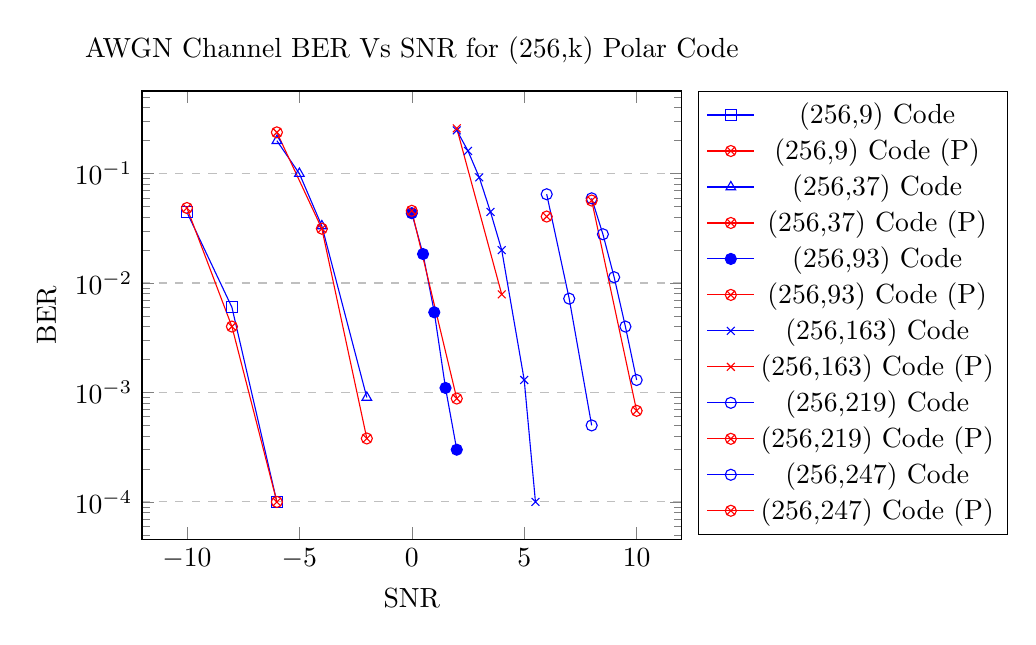
\begin{tikzpicture}
\begin{semilogyaxis}
[
    title={AWGN Channel BER Vs SNR for (256,k) Polar Code},
    xlabel={SNR},
    ylabel={BER},
    % xmin=0, xmax=1.0,
    % ymin=0, ymax=0.5000,
    % xtick={0.10,0.20,0.30,0.40,0.50,0.60,0.70,0.80,0.90,1.00},
    % ytick={0.00,0.050,0.100,0.150,0.250,0.300,0.350,0.400,0.450,0.500},
    legend pos=outer north east,
    ymajorgrids=true,
    grid style=dashed,
]
 
    \addplot[
    color=blue,
    mark=square,
    ]
    coordinates {
    (-10.0,0.0443)(-8.0,0.0060)(-6.0,0.0001)(-4.0,0.00)(-2.0,0.00)(0.00,0.00)(2.0,0.00)(4.0,0.00)(6.0,0.00)(8.0,0.00)(10.0,0.00)
    };
    \addlegendentry{(256,9) Code}
    
    \addplot[
    color=red,
    mark=otimes,
    ]
    coordinates {
    (-10.0,0.04844)(-8.0,0.0040)(-6.0,0.0001)(-4.0,0.00)(-2.0,0.00)(0.00,0.00)(2.0,0.00)(4.0,0.00)(6.0,0.00)(8.0,0.00)(10.0,0.00)
    };
    \addlegendentry{(256,9) Code (P)}
    

    \addplot[
    color=blue,
    mark=triangle,
    ]
    coordinates {
    (-6.0,0.1996)(-5.0,0.0999)(-4.0,0.0332)(-2.0,0.0009)(0.00,0.00)(2.0,0.00)(4.0,0.00)(6.0,0.00)(8.0,0.00)(10.0,0.00)
    };
    \addlegendentry{(256,37) Code}
    
    \addplot[
    color=red,
    mark=otimes,
    ]
    coordinates {
    (-6.0,0.23784)(-4.0,0.03135)(-2.0,0.00038)(0.00,0.00)(2.0,0.00)(4.0,0.00)(6.0,0.00)(8.0,0.00)(10.0,0.00)
    };
    \addlegendentry{(256,37) Code (P)}
    
    \addplot[
    color=blue,
    mark=*,
    ]
    coordinates {
    (0.00,0.0434)(0.5,0.0184)(1.0,0.0054)(1.5,0.0011)(2.0,0.0003)(4.0,0.00)(6.0,0.00)(8.0,0.00)(10.0,0.00)
    };
    \addlegendentry{(256,93) Code}
    
    \addplot[
    color=red,
    mark=otimes,
    ]
    coordinates {
    (0.00,0.04568)(2.0,0.00088)(4.0,0.00)(6.0,0.00)(8.0,0.00)(10.0,0.00)
    };
    \addlegendentry{(256,93) Code (P)}
    
    \addplot[
    color=blue,
    mark=x,
    ]
    coordinates {
    (2.0,0.2480)(2.5,0.1609)(3.0,0.0923)(3.5,0.0446)(4.0,0.0200)(5.0,0.0013)(5.5,0.0001)(6.0,0.00)(8.0,0.00)(10.0,0.00)
    };
    \addlegendentry{(256,163) Code}
    
    \addplot[
    color=red,
    mark=x,
    ]
    coordinates {
    (2.0,0.25902)(4.0,0.00787)(6.0,0.00)(8.0,0.00)(10.0,0.00)
    };
    \addlegendentry{(256,163) Code (P)}
 
    \addplot[
    color=blue,
    mark=o,
    ]
    coordinates {
    (6.0,0.0647)(7.0,0.0072)(8.0,0.0005)(9.0,0.000)(10.0,0.000)
    };
    \addlegendentry{(256,219) Code}
    
    \addplot[
    color=red,
    mark=otimes,
    ]
    coordinates {
    (6.0,0.04048)(8.0,0.0)(10.0,0.000)
    };
    \addlegendentry{(256,219) Code (P)}
    
    \addplot[
    color=blue,
    mark=o,
    ]
    coordinates {
    (8.0,0.0594)(8.5,0.0279)(9.0,0.0113)(9.5,0.0040)(10.0,0.0013)
    };
    \addlegendentry{(256,247) Code}
    
    \addplot[
    color=red,
    mark=otimes,
    ]
    coordinates {
    (8.0,0.05671)(10.0,0.00068)
    };
    \addlegendentry{(256,247) Code (P)}
    
\end{semilogyaxis}
\end{tikzpicture}

\section{Doubt}
Consider the following step in the algorithm from the paper \cite{hooshmand2013secret}
\begin{equation}\label{eq:12}
\tilde{C}*P^{T} - Z_{ie}*P^{T}  = M^{'}*G_{A} + Z_{ce}*P^{T}
\end{equation}

where $Z_{ce}$ is channel error, the right hand side is obtained using the received vector and the secret key. \newline

In polar coding, if my understanding is correct, $M^{'} = M*S$ is transmitted through the good channels which is accomplished through $G_{A}$. Implying the errors are added in the bad channels which is represented by $Z_{ce}$. When $Z_{ce}$ is multiplied by $P^{T}$ in \ref{eq:12} some of the errors may be permuted to good channels resulting in decoding error and if $P^{T}$ is chosen incorrectly then most of the errors can be permuted to the good channels. \newline

For example, let $G = \begin{bmatrix}
    1       & 0 & 0 & 0 \\
    1       & 0 & 1 & 0 \\
    0       & 0 & 1 & 0 \\
    1       & 1 & 1 & 1
\end{bmatrix} $ $M^{'} = [1 0 0 0]$. Let the rate $R = 1/2$ with $N=4, k=2$ and based on the Bhattacharya parameter $A = \{3, 4\}$, then $A^{c}=\{1, 2\}$, is obtained. $Z_{ce}$ is $[1 1 0 0]$, $[0 1 0 0]$ and $[1 0 0 0]$, other errors having low chances. If $P^{T} = \begin{bmatrix}
    0       & 0 & 1 & 0 \\
    0       & 0 & 0 & 1 \\
    1       & 0 & 0 & 0 \\
    0       & 1 & 0 & 0
\end{bmatrix}$ then $Z_{ce}*P^{T}$ is $[0 0 1 1]$, $[0 0 0 1]$ and $[0 0 1 0]$, leading to addition of errors in good channels i.e, $A = \{3,4\}$.

\section{Concerns}
Can a budget be allocated for providing a laptop?

\bibliographystyle{unsrtnat}
\bibliography{ref}
\end{document}
